\documentclass[12pt]{article}
  \usepackage[francais]{babel}
  \AddThinSpaceBeforeFootnotes % à insérer si on utilise \usepackage[french]{babel}
  \FrenchFootnotes % à insérer si on utilise \usepackage[french]{babel}
  \usepackage[T1]{fontenc}
  \usepackage[utf8]{inputenc}
  \usepackage{graphicx}
  \usepackage[left=2.5cm,right=2.5cm,top=2.5cm,bottom=2.5cm]{geometry}
  \usepackage{array}
  \usepackage{booktabs}
  \usepackage[squaren,Gray]{SIunits}  % Unité ex: $\unit{5 \cdot 10^{-6}}{\meter}$
  \usepackage{colortbl}               % Pour les couleur des cellules (tableau)
  \usepackage{amsmath}				  % Pour les formules mathématiques
  \usepackage{upgreek}                % Pour les lettres greque
  %\usepackage{fullpage}	          % plus petites marges
  \usepackage{verbatim}				  % Pour de long commentaires
  \usepackage[lofdepth,lotdepth]{subfig}       % Faire des sous-figures
  \usepackage{url}
  \usepackage{colortbl}               % pour les couleur des cellules (tableau)
  \usepackage{indentfirst}
  \usepackage{multirow}
  \usepackage{xfrac}
  \usepackage{wrapfig}
  \usepackage{enumitem}               % Liste personnalisée
  \frenchbsetup{StandardLists=true}   % Empêche conflits entre enumitem et babel
  \usepackage{placeins}   % place une barrière pour que l'image/table soit derrière \FloatBarrier
  \usepackage{lastpage} 
  \usepackage{titling}
  \usepackage{lmodern}
  \usepackage{booktabs}
  \usepackage{etoolbox}
  \usepackage[most]{tcolorbox}
  
  
  %Change la taille de police
  \newcommand\ChangeRT[1]{\noalign{\hrule height #1}}
  
\graphicspath{{images/}}

  
  %Création  d'une nouvelle commande pour faire référence à une Figure
  %Exemple : \appelFigure{schema} donne : Figure 1 (en italique)
  \newcommand{\appelFigure}[1]{
    \textit{Figure \ref{#1}}
  }
      
  %%Création commande pour insérer image avec nom de figure directement
  %\newcommand{nomDeTaCommande}[nombreArguments]{CodeLaTeX}
  %\insertImage[position]{image_path}{scale}{Titre_figure}{label}
  \newcommand{\insertImage}[5][center]{
      \begin{#1}
      \includegraphics[scale=#3]{#2}
      \captionof{figure}{#4} 
      \label{#5}
      \end{#1}
  }

  % Affichage des frames pour commande cisco
  \newtcblisting{cisco}[1][]{size=fbox, listing only, listing options={style=tcblatex,basicstyle=\ttfamily\scriptsize,tabsize=2,language=sh},title=#1}

  %En-tête et pied de page personalisé
  \usepackage{fancyhdr}
  \pagestyle{fancy}
  \fancyhf{}
  \setlength\parindent{0pt} %Supprime les alinéa
  \setlength{\parskip}{8pt} %Augmente l'espace entre paragraphe
  %Bottom numbering page
  \renewcommand{\headrulewidth}{1pt}
  \fancyhead[L]{
\includegraphics[scale=.2]{heia-fr-logo.png}}
  \fancyhead[R]{\theauthor}
  
  \renewcommand{\footrulewidth}{1pt}
  \fancyfoot[R]{\textbf{Page \thepage\ sur \pageref{LastPage}}} 
%  \fancyfoot[L]{\leftmark}

  \setlength\parindent{0pt} %Supprime les alinéa
  \setlength{\parskip}{8pt} %Augmente l'espace entre paragraphe

 
\title{Résumé OS de mort} 
\author{\textsl{Marc} \textsc{Roten}}
\date{}



\begin{document}
    \begin{titlepage}
        \begin{center}
            
\includegraphics[scale=.4]{Img/heia-fr-logo.png}\\[1.3cm]
            
            \rule{\linewidth}{0.3mm} \\[0.3cm]
            {\huge \bfseries Operating Systems\\[0.5cm]} 
            {\Large  Résumé TE02 }
            \rule{\linewidth}{0.3mm} \\[0.8cm]
            \noindent{}
            \begin{minipage}[t]{0.4\textwidth}
                \begin{flushleft} \large
                    \emph{Auteur :}\\
                    \theauthor
                \end{flushleft}
            \end{minipage}
            \begin{minipage}[t]{0.4\textwidth} 
                \begin{flushright} \large
                    \emph{Professeur:}\\
                    \textsl{Jacques} \textsc{ Supcik}\\ 
                \end{flushright} 
                \vfill
            \end{minipage}\\[1.3cm]
            
\includegraphics[scale=0.3]{Img/title.jpg}\\[1.5cm]
            \vspace*{1\baselineskip}
            \today \\[0.7cm]
        \end{center}
    \end{titlepage}
    \tableofcontents
    \clearpage 
% \insertImage{Img/photo.PNG}{0.8}{Schéma explicatif}{}

% \section{voici comment faire un chapitre}

%     \subsection{Voici comment faire un sous chapitre}

% \section{des commandes}
%     \subsection{commande cisco}
    
%     \begin{cisco}[une commande sympa type cisco]
%       un texte lambda
%     \end{cisco}
    
%     \subsection{commande cisco allégée}
    
%     \begin{cisco}
%       un texte lambda
%     \end{cisco}
    
    
%     \subsection{commande pour mettre une image}
    
%     % \insertImage{Img/1.PNG}{echelle pour l'image (source = 1)}{texte dessous l'image}{référence vers l'objet
%     \insertImage{Img/1.JPG}{0.6}{voici une image}{myImg}
%       \insertImage{Img/27.JPG}{0.6}{}{}

\section{Introduction}
Résumé pour la deuxième inter d'OS. Spécial dédicace à ma mère, pour la fête des mères.\\[5.5cm]
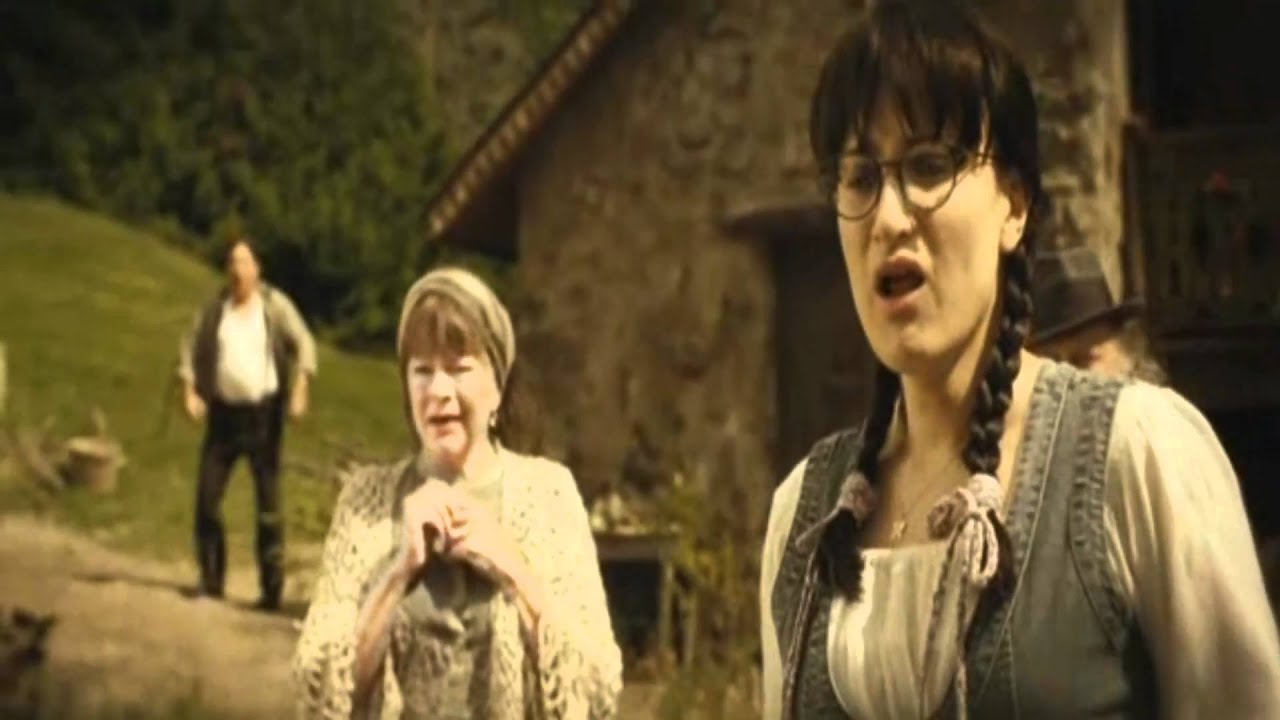
\includegraphics[scale=.35]{Img/0.PNG}
\newpage
\section{Chapitre\_6 La Gestion de la Mémoire}

















\newpage
\section{Chapitre\_7 Systèmes de fichiers}

\subsection{Exigences stockage long terme}
Pour tout ce qui concerne le stockage à long terme, il y a trois exigences.
\begin{itemize}
    \item \textbf{Grande capacité de stockage: } on doit pouvoir enregistrer une grande quantité d'information
    \item \textbf{Persistance: }L'information, les modifications mémoires doivent persister après l'arrêt du processus qui les utilise
    \item \textbf{Mémore partagée: }Plusieurs processus doivent pouvoir accéder en même temps à la même information.
\end{itemize}

\subsection{Le disque magnétique HDD}
Le disque peut être considéré comme une suite séquentielle de blocs de taille fixe. Un disque possède deux opérations:
\begin{itemize}
    \item lire un bloc K
    \item écrire un bloc K
\end{itemize}

\subsection{Abstraction supplémentaire: le FICHIER}
De tout temps, en informatique, pour simplifier l'utilisation et l'accès aux données, on a rajouté un niveau d'abstraction au niveau de l'OS, via ce que l'on appelle couramment : \textbf{File System.} c'est la partie qui gère les fichiers.
\insertImage{Img/1.PNG}{0.7}{Liste non exhaustive des différents File System}{FS}.

Chaque \textbf{File System} définit ses propres rêgles concernant les noms de fichiers:
\begin{itemize}
    \item Caractères autorisés
    \item encodage (ISO, Latin 1, UTF-8/16)
    \item nb Max
    \item distinction minuscule et majuscule
\end{itemize}

\subsubsection{systéme FAT}
Le système FAT définit la convention «8.3» :
\begin{itemize}
    \item 8 caractères pour le nom  du fichier, 3 pour l'extension
    \item encodage sur 8 bit 
    \item Les caractères interdits
    \item espaces autorisés
    \item pas de distinction entre minuscule et majuscule
\end{itemize}

\subsubsection{NTFS-EXT}
\insertImage{Img/2.PNG}{0.7}{NTFS EXT}{NTFS}

\subsection{Les extensions}

\textbf{Extension de nom de fichier: }Suffixe ajouté au nom d'un fichier pour identifier son format.

Chaque système (Windows ou UNIX) ne gère pas les extensions de manière simillaire. Voire ci-dessous

\begin{itemize}
    \item \textbf{UNIX: }L'extension est juste une concention. exemple: fichier peut se nommer .vhd mais être un fichier executable. 
    \item \textbf{UNIX: }Possible d'avoir plusieurs extension comme par exemple archive.tar.gz
    \item \textbf{Windows: }les extensions sont associées au programme qui peur traiter lesfichiers correspondants.
\end{itemize}

\insertImage{Img/3.PNG}{0.7}{extensions courantes}{ext}

\subsection{La structure des fichiers}
Il existe trois sortes de fichiers:
\begin{itemize}
    \item Suite d’octet (byte sequence)
    \item Suite d’enregistrements (record sequence)
    \item Arbre (tree)
\end{itemize}

\subsection{Commandes spéciales}
Commande trouver les fichiers caractères: $find / dev / - type$ $c$

Commande trouver les fichiers spéciaux blocs:  $find / dev / - type$ $b | column -c$ $67 | expand$

\subsection{Fichiers Ordinaires}
\subsubsection{Texte}
\begin{itemize}
    \item Encodage des caractères (ASCII, ISO/IEC 8859-1/Latin1, UTF-8,UTF-16, …)
    \item Conventions pour coder la fin d’une ligne (End Of Line – EOL).
\end{itemize}

\textbf{Caractères communs retout à la ligne} ci-dessous
\insertImage{Img/4.PNG}{0.6}{CR LF }{R}

\subsubsection{Binaire}

\insertImage{Img/5.PNG}{0.65}{fichiers Binaires}{BN}
\begin{itemize}
    \item (a) un fichier executable
    \item (b) un fichier d'archive
\end{itemize}

\subsection{Les nombres magiques}
Les nombres magiques sont utilisés par les programmes pour identifier un fichier. Voir liste en Figure \ref{mn}

\insertImage{Img/6.PNG}{0.65}{Chiffres magiques}{mn}

\subsection{L'accès aux fichiers sequantial/random}
\textbf{\textit{Sequential Access}}:Ce système est utilisé principalement pour les bandes magnétique

\textbf{\textit{Random Access}}: Utilisé principalement par les disques. Ce système permer un déplacement à une position donnée. \textbf{Fonction SEEK}
\subsection{Attributs supplémentaires}

\insertImage{Img/7.PNG}{0.65}{Attributs supplémentaires}{att}

\subsection{Appels systèmes: Opérations sur les fichiers}
systems Calls
\begin{itemize}
    \item \textbf{Create: } RAJOUTER DU MERDIER
    \item \textbf{Delete}
    \item \textbf{Open}
    \item \textbf{close}
    \item \textbf{read}
    \item \textbf{write}
    \item \textbf{Append}
    \item \textbf{SEEK}
    \item \textbf{get attributes}
    \item \textbf{Set attributes}
    \item \textbf{rename}

\end{itemize}
Toutefois, on constate qu'il n'y a pas de COPY. La fonction copy n'est pas présente parceque:................................... Ci dessous voici l'implémentation de la fonction copy.\\[.5cm]

\begin{lstlisting}
    copy ( source , destination )

sf = open ( source ) # sf is a file descriptor
df = create ( destination ) # df is a file descriptor
buffer_size = 4096
buffer = array [ buffer_size ] of byte
while true :
    count = read (sf , buffer , buffer_size )
    if count <= 0:
        break
    write (df , buffer , count )
close ( sf )
close ( df )
\end{lstlisting}










\newpage
\section{Chapitre\_8 Systèmes de Fichiers / Répertoires}

















\newpage
\section{Chapitre\_9 Disques / Systèmes de Fichiers}














































\newpage
\section{Conclusion}
Si vous avez aimé mon résumé, faites un git clone de mon Git. Suivez moi sur gitlab.forge.heia-fr.ch github and iLoveFreeSoftware.com.


\end{document}